 \documentclass[12pt,a4paper]{article}
\author{Walid Laouidji}
\title{  \sffamily
  رسم جداول الوضعية النسبية بين منحنى و مستقيم
\hfill \\
\LR{\ttfamily{Version : 2.1  }}
  }
 %
\begin{document}
 
 \maketitle
 \hrulefill
 \tableofcontents
 \hrulefill
 
 \vspace{2cm}
 \section{إدراج الحزمة}
{\begin{naam cadre}{نبذة عن الحزمة
 \hfill
الحزمة
\texttt{na-position}}
 \texttt{na-position} 
 تعتمد أساسا على 
الحزمة
 \texttt{tkz-tab}  
.
بعد تحميل الحزمة   
 \texttt{na-position}
 من الرابط 
: 
\\
\url{https://github.com/WaliDLw/tkz-pos/archive/master.zip}
\\
 يجب عليك تثبيتها
 على
 \texttt{Live TeX} 
أو على
 \texttt{Miktex}
.\\
إن لم تتمكن من ذلك ضعها في نفس مجلد ملف المصدر الذي تكتب فيه.
  \\
   الحزمة
    \texttt{na-position}
تعمل مع الحزمة
 \texttt{polyglossia}  
عند المعالجة بآلية 
  \texttt{\XeLaTeX}. 
 \end{naam cadre}}
\newpage
 \section{إشارة الفرق $f(x)-y$ }
 \begin{itemize}
 \item
 نستعمل
 \LR{\texttt{$\backslash$tkzTabLine}}
 لادراج اشارة الفرق
 $f(x)-y$
 في جدول الوضع النسبي . 
 \item
 إذا كان 
 $\Nplot$
 فوق
 $\Nline$
 نضع الإشارة 
 $+$
 .
 \item
 أما
  إذا كان 
 $\Nplot$
 تحت
 $\Nline$
 نضع الإشارة 
 $-$.
  \end{itemize}
  
\begin{tikzpicture}[overlay,xshift=-1.3cm,yshift=2.2cm]
\tkzTabInit[espcl=4]
{$x$/1,
$f(x)-y$ /1.5}%
{ , ,}%
\tkzTabLine{ ,  ,  ,  , }
\node[draw,inner sep=2pt,circle,fill=red!20] at (Z11) {$1$} ;
\node[draw,inner sep=2pt,circle,] at (S11) {$\pm$} ;
\node[draw,inner sep=2pt,circle,fill=red!20] at (Z21) {$2$} ;
\node[draw,inner sep=2pt,circle,] at (S21) {$\pm$} ;
\node[draw,inner sep=2pt,circle,fill=red!20] at (Z31) {$3$} ;
\node[,inner sep=2pt,rectangle,fill=green!20] at (F0) {$x$} ;
\node[,inner sep=2pt,fill=green!20] at (F1) {$f(x)-y$} ;
\node[,inner sep=1pt,fill=blue!10,xshift=0.5cm] at (L1) {{\scriptsize \RL{الطرف الأول}}} ;
\node[,inner sep=1pt,fill=blue!10,xshift=0.1cm] at (L2) {$\alpha$} ;
\node[,inner sep=1pt,fill=blue!10!white,xshift=-0.4cm] at (L3) {{\scriptsize \RL{الطرف الثاني}}} ;
\end{tikzpicture}
 
 \begin{enumerate} 
\item[•]
عندما يكون الطرف الأول من المجال مفتوحا عند عدد حقيقي 
\textcolor{red}{$a$}
 نضع الرمز :
{\textcolor{blue}{ $\rm d$}}
، وعندما يكون 
$-\infty$\\
أو مغلقا نترك مكان الرقم 
\,
\tikz[overlay]\node[,yshift=0.1cm,draw,inner sep=1pt,circle,fill=red!10]{$1$};
\,
فراغا. 
\item[•]
إذا كانت
\textcolor{red}{$\alpha$}
نقطة التقاطع نضع الرمز
{\textcolor{blue}{ $\rm z$}}
، بينما إذا كانت 
\textcolor{red}{$\alpha$}
قيمة ممنوعة 
 نضع الرمز
{\textcolor{blue}{ $\rm d$}}
.
\item[•]
عندما يكون الطرف الثاني من المجال مفتوحا عند عدد حقيقي 
\textcolor{red}{$b$}
 نضع الرمز :
{\textcolor{blue}{ $\rm d$}}
،
وعندما يكون 
$+\infty$\\
أو مغلقا نترك مكان الرقم 
\, 
\tikz[overlay]\node[,yshift=0.1cm,draw,inner sep=1pt,circle,fill=red!10]{$3$};
\,
فراغا. 
\end{enumerate}



\begin{boxe}{ مثال}
%\usepackage{na-position}
\begin{tikzpicture}
\tkzTabInit[espcl=2] {$x$/1,$f(x)-y$/1}
{$-\infty$ , $1$, $+\infty$ }
\tkzTabLine{,+,z,-,} 
\end{tikzpicture}
\end{boxe}
%\newpage
\begin{boxe}{ مثال}
\begin{tikzpicture}
\tkzTabInit[espcl=2] {$x$/1,$f(x)-y$/1}
{$-\infty$ , $-2$,$2$, $+\infty$ }
\tkzTabLine{,-,z,+,z,-} 
\end{tikzpicture}
\end{boxe}
%
\newpage
\section{التعليمة \LR{\texttt{$\backslash$tkzTabPos}}}
\begin{itemize}
\item
لها نفس مبدأ عمل التعليمة
 \LR{\texttt{$\backslash$tkzTabLine}}
 الخاصة بحزمة 
 \texttt{tkz-tab}.
 \item
 لإضافة سطر الوضع النسبي نكتب الأمر
 \LR{\texttt{$\backslash$tkzTabPos}}
 تحت
 الأمر 
 \LR{\texttt{$\backslash$tkzTabLine}}.
 
\begin{boxe}{مثال}
\begin{tikzpicture}
\tkzTabInit[espcl=2] {$x$/1,$f(x)-y$/1,~\textarabic{الوضع النسبي}~/2} 
{a,b,c}
\tkzTabLine{, , ,}
\tkzTabPos{, , ,} 
\end{tikzpicture}
\end{boxe}
\item
ندرج اشارة الفرق 
$f(x)-y$
كما فعلنا سابقا
  ،
  نضع نفس الاشارات التي كتبناها
  داخل
 \LR{\texttt{$\backslash$tkzTabLine}}  
  في
    \LR{\texttt{$\backslash$tkzTabPos}}.
\item
إذا كان هناك نقطة أو نقاط تقاطع بين المنحى والمستقيم
نضع الرمز
:
\fbox{\textenglish{\textcolor{blue}{$\rm z$}
{\textcolor{red}{\Large /}}\textcolor{blue}{\textarabic{نقطة التقاطع}}}}
داخل التعليمة
\LR{\texttt{$\backslash$tkzTabPos}}.
\end{itemize}


\begin{boxe}{مثال}
 \begin{tikzpicture}
\tkzTabInit[espcl=2]{$x$/1,$f(x)-y$/1,~\textarabic{الوضع النسبي}~/2 }%
{$-\infty$ , $1$, $+\infty$ }%
\tkzTabLine{,+,z,-,}
 \tkzTabPos{ ,+,z/$\left(1;f(1)\right)$ ,-,} 
\end{tikzpicture}
\end{boxe}

\begin{boxe}{مثال}
\begin{tikzpicture}
\tkzTabInit[espcl=3]{$x$/1,$f(x)-y$/1,~\textarabic{الوضع النسبي}~/2 }
{$-\infty$ , $-3$ , $3$, $+\infty$ }%
\tkzTabLine{t,+,z,-,z,+,t }
\tkzTabPos{t,+,z/$A(-3;f(-3))$ ,-,z/$A(3;f(3))$,+,t}%
\end{tikzpicture}
\end{boxe}

\begin{boxe}{مثال}
\begin{tikzpicture}
\tkzTabInit[espcl=2]{$x$/1,$f(x)-y$/1,~\textarabic{الوضع النسبي}~/2 }
{$-\infty$ , $-3$ , $3$, $5$ ,$+\infty$ } 
\tkzTabLine{t,+,d,h,d,+,z,-, }
\tkzTabPos{t,+,d,h,d,+, z/$A\left(5;f(5)\right)$,-,} 
\end{tikzpicture}
\end{boxe} 
{\section{تغيير اسم المنحنى واسم المستقيم}
\begin{boxlis}
*\begin{flushright}
\textarabic{نضيف الأمر :
 }
\end{flushright}*
\def\Nplot{*\textarabic{اسم المنحنى
 }*}
\def\Nline{*\textarabic{اسم المستقيم
 }*}
\end{boxlis}}
\begin{boxe}{ مثال }
\def\Nplot{(C_g)}
\def\Nline{(T)}
\begin{tikzpicture}
\tkzTabInit[espcl=3]{$x$/1,$g(x)-y$/1,~\textarabic{الوضع النسبي}~/2 }
{$-\infty$ , $-\sqrt{3}$ , $3$, $+\infty$ }%
\tkzTabLine{t,+,z,-,z,+,t }
\tkzTabPos{t,+,z/$A(-\sqrt{3};g(-\sqrt{3}))$ ,-,z/$A(3;g(3))$,+,t} 
\end{tikzpicture}
\end{boxe}
\section{تغيير شكل ولون خط التقاطع}
لتغيير شكل خط التقاطع إلى
{\ttfamily{dotted}}
،
{\ttfamily{dashed}}
أو
{\ttfamily{double}}
نضيف الأمر :
{\begin{boxlis}
\tikzset{pos style/.append style={*\textarabic{نمط الخط}*}}
\end{boxlis}}
\begin{boxe}{ مثال خط متقطع ولونه أحمر}
\tikzset{pos style/.append style={dashed,red}}
\begin{tikzpicture}
\tkzTabInit[espcl=3]{$x$/1,$f(x)-y$/1,~\textarabic{الوضع النسبي}~/2 }
{$-\infty$ , $-3$ , $3$, $+\infty$ }%
\tkzTabLine{t,+,z,-,z,+,t }
\tkzTabPos{t,+,z/$A(-3;f(-3))$ ,-,z/$A(3;f(3))$,+,t} 
\end{tikzpicture}
\end{boxe}
 \end{document}
 